\section{State of the Art image reconstruction}\label{state}
We present here state of the art deconvolution algorithms.
All implemented in the WSCLEAN software package.
The two state-of-the-art deconvolution algorithms will be compared to our serial and parallel coordinate descent algorithms later in Section \ref{results} on a real-world MeerKAT observation.


\subsection{Multi-scale CLEAN}
We introduced the standard CLEAN algorithm in the previous Section \ref{intro2:CLEAN}.  Multi-scale CLEAN is an extension of the standard CLEAN algorithm. The extension allows for accurate modeling of extended emissions. The standard CLEAN algorithm has difficulties reconstructing extended emissions accurately: It assumes the image consists of point sources. When it encounters an extended emission, it simply approximates it with a cloud of point sources. 

Multi-scale CLEAN solves this issue. It deconvolves the image at different resolutions (scales). The new algorithm consists of two parts: It first selects a scale (resolution) to deconvolve the dirty image. Then it performs several standard CLEAN iterations at the selected scale. If it selects the lowest scale, the CLEAN iterations are identical to standard CLEAN and point sources are added to the model image. However, if it selects a higher scale, it then adds a 2d Gaussian shaped emissions to the model image.

In pseudo-code, the multi-scale CLEAN idea leads to the following algorithm:
\begin{lstlisting}
dirtyImage = iFFT(Gridding(visibilities))
model = new Array[,]

do
	//select a scale. Large scales mean lower resolutions
	selectedScale = 0
	selectedMaxValue = 0
	for each scale in scales
		scaledDirty = Convolve(dirty, Gaussian(scale))
		maxValue = Max(scaledDirty) * ScaleBias(scale)
		if(selectedMaxValue < maxValue)
			selectedMaxValue = maxValue
			selectedScale = scale
			
	//standard CLEAN iteration, but the dirty image gets blurred
	scaledDirty = Convolve(dirty, Gaussian(scale))
	scaledPSF = Convolve(PSF, Gaussian(scale))
	scaledModel = CLEAN(scaledDirty, scaledPSF)
	
	//update dirty and model image
	standardModel = Convolve(scaledModel, Gaussian(scaledModel))
	model = model + standardModel
	dirtyImage = dirtyImage - Convolve(standardModel, PSF)
while
\end{lstlisting}

Note the scale-bias function: Modern multi-scale CLEAN implementations prioritize the scales, which improves the reconstruction quality \cite{offringa2017optimized}. Usually, the larger scales are prioritized before the lowest scale, where the algorithm is adding point-sources to the model image. 

This is the multi-scale CLEAN algorithm widely used for radio interferometric reconstructions.
Non-zero pixels
Various Improvements and speedups, but the core algorithm is still this.

\subsection{MORESANE}
MOdel REconstruction by Synthesis ANalasys Estimators (MORESANE) is another multi-scale deconvolution algorithm used in radio astronomy. Instead of deconvolving the image at different scales like multi-scale CLEAN, MORESANE uses a regularization with multi-scale built into it. It uses the starlet transform \cite{starck2015starlet} as regularization.

\begin{figure}[h]
	\centering
	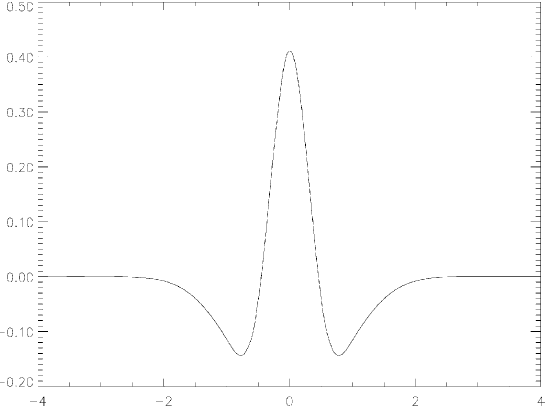
\includegraphics[width=0.3\linewidth]{./chapters/02.state/wavelet.png}
	\caption{The starlet wavelet in one dimension}
	\label{state:moresane:starlet}
\end{figure}

The starlet transform represents an image as a combination of starlet wavelets (shown in Figure \ref{state:moresane:starlet}) at different locations and scales. At the lowest scale, each starlet wavelet is a single pixel wide. At larger scales, each starlet wavelet spans over several pixels. It is an over-complete representation, because we can use several different combinations of starlet wavelets at different scales that lead to the same image.

Normally, we can only retrieve the image from the over-complete representation and not the other way around (because there are different combinations of starlets that lead to the same image). The starlet transform has a way to estimate its wavelet components from the dirty image. The MORESANE algorithm uses this property for reconstruction.

\begin{lstlisting}
dirtyImage = iFFT(Gridding(visibilities))
starlets = new Array[x, y, scale]

do
	//estimate starlet components,
	estimates = StarletTransform(dirtyImage, PSF)
	maxIndex = ArgMax(estimates)
	
	//find connected starlet components. Flood fill over the image(x, y) and over scales. Now we should have all starlets belonging to a single object (e.g. a hydrogen cloud or a single galaxy in the image)
	connectedStarlets = FloodFill(starlets, maxIndex)
	
	optimizedStarlets = ConjugateGradients(dirtyImage, connectedStarlets)
	
	//update dirty image and our starlet model
	starlets = starlets + optimizedStarlets
	standardModel = Sum(optimizedStarlets, axis=scale)
	dirtyImage = dirtyImage - Convolve(standardModel, 
while

model = Sum(starlets, axis=scale)
\end{lstlisting}

First, it uses the starlet transform on the dirty image, and search for the largest starlet component at a certain scale. The largest starlet component explains part of a single object emitting radio waves, like a hydrogen cloud or a galaxy. Next, we use the flood-fill algorithm to find all starlet components at all scales which describe this object.

The next step is the actual minimization step in the MORESANE algorithm: We use the conjugate gradient method and find 

Starlets 

Uses the starlet wavelet 

Generally produces better results than multi-scale CLEAN, but is less robust versus calibration errors.

The basic algorithm is??




